%================================================================== %
\begin{frame}
	\begin{figure}
		\centering
		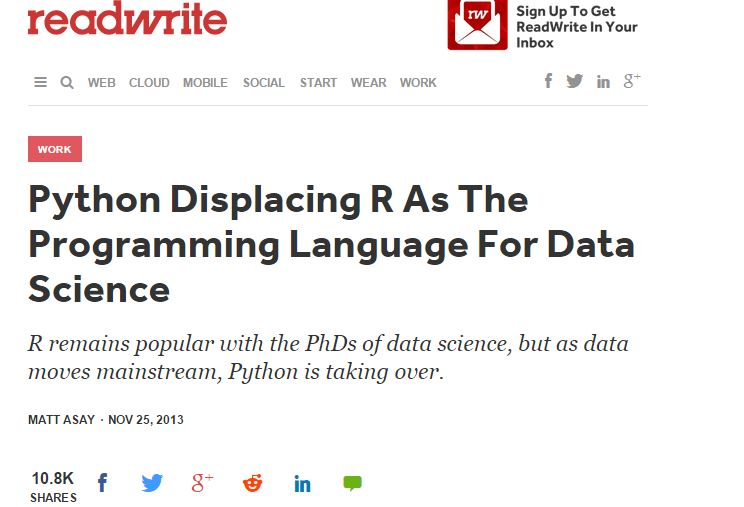
\includegraphics[width=1.05\linewidth]{mjasay}
		
	\end{figure}
	
\end{frame}
\begin{frame}
	\begin{figure}
		\centering
		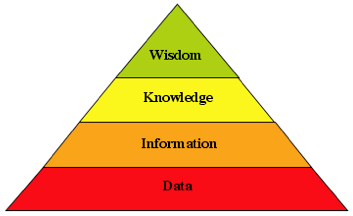
\includegraphics[width=0.9\linewidth]{KnowledgePyramid}
		
	\end{figure}
	
\end{frame}


%===========================================================%
\begin{frame}
\frametitle{matplotlib and seaborn}
\large
	\vspace{-0.4cm}
\textbf{Graphics Packages}
\begin{itemize}
\item \textbf{matplotlib} provides a plotting environment for 2D plots, with limited support for 3D plotting. 
\item \textbf{seaborn} is
a Python package that improves the default appearance of matplotlib plots without any additional code.
\end{itemize}

\end{frame}
%===========================================================%
\begin{frame}
\frametitle{pandas}
\Large
\begin{itemize}
\item 	\textit{pandas} is a high-performance module that provides a comprehensive set of structures for working with
data. 
\item \textit{pandas} excels at handling structured data, such as data sets containing many variables, working with
missing values and merging across multiple data sets. 
\end{itemize}
\end{frame}
%===========================================================%

%===========================================================%
\begin{frame}
	\large
	\frametitle{pandas}	
	\large
	\begin{itemize}
	
	\item While extremely useful, \textit{pandas} is not an essential component of the Python scientific stack unlike NumPy, SciPy or matplotlib, and so while \textit{pandas} doesn’t
	make data analysis possible in Python, it makes it much easier. \item \textit{pandas} also provides high-performance,
	robust methods for importing from and exporting to a wide range of formats.
	\item - example \texttt{read.csv()}
	\end{itemize}
\end{frame}
\begin{frame}


\end{frame}